\section{Relation Vocabulary Raises Held-Out QA}
\label{sec:res-schema}

The relation list raised held-out grounded QA in all four Exp7 pipelines of Qwen on 2Wiki (Table~\ref{tab:exp8}\figseedref). L0 gained 14.7 points ([10.9, 18.4]), LOOP 9.4, the combined pipeline 9.3 and U-ext 4.5, a range of 4.5 to 14.7. The arms are defined in Table~\ref{tab:arms}. In Gemma on 2Wiki the list raised grounded QA over no list by 7.4 points in L0 ([3.3, 11.3]) and 7.5 in LOOP ([1.3, 15.0]). The Gemma combined pipeline gained 9.3 ([5.7, 12.9]). Further contrasts with their status are in Appendix Table~\ref{tab:glance}.

\IfFileExists{figures/fig_seed_forest_r62.pdf}{%
\begin{figure}[t]
\centering
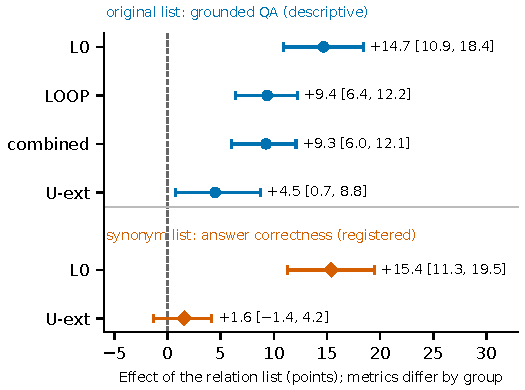
\includegraphics[width=\columnwidth]{figures/fig_seed_forest_r62.pdf}
\caption{The relation list raised held-out grounded QA in all four pipelines, and synonym names raised answer correctness in L0. Differences in points with 95\% intervals, Qwen on 2Wiki. The two groups use different metrics. Top, original list: grounded QA, descriptive. Bottom, synonym list: answer correctness, registered; L0 +15.4 [11.3, 19.5], U-ext +1.6 [$-$1.4, 4.2].}
\label{fig:seedforest}
\end{figure}}{}

Synonym names kept the benefit in L0. No question ID or normalised question text of the list's training split appears among the evaluation questions. No synonym shares a word stem with its original name. In L0 answer correctness rose by 15.4 points (Qwen, 2WikiMultihopQA; [11.3, 19.5], Holm $p$ = 0.0002; Table~\ref{tab:synseed}), and grounded QA rose by 15.8 ([11.5, 20.3]). In U-ext, which already extracts from every chunk, the gain was +1.6 ([$-$1.4, 4.2]), in line with the smaller effect of the original list there (Appendix Table~\ref{tab:seedalign}).

In L0 the synonym list's answer correctness was within 1.7 points of the original list's ([$-$2.0, 5.0]), while the original list gained 13.8 over no list in the stored runs.

A list induced from the corpus, with no gold relations, raised L0 answer correctness by 16.3 points ([11.6, 20.2], Holm $p$ = 0.001, registered). The original list rerun on the same instance gave +15.1 ([10.5, 19.5]); the same arm differed between serving instances (no list .433 stored, .417 rerun), so contrasts are taken within one instance where possible.

The same induction on T-REx, from 300 of that corpus's 386 documents, gave a list of 22 names. No question and no gold relation was used. There it raised the single pass by 13.3 points of grounded QA ([8.0, 23.1], registered: improved) and by 12.5 points of answer correctness (registered: improved, Table~\ref{tab:trexseed}).

A second T-REx list, induced from 96 passages outside the evaluation shards with the same procedure and no question, shares 15 of its 22 names with the first and 6 with the 2Wiki list. With this outside-shard list, the single pass scored 7.4 points above no list in grounded QA ([3.9, 11.4], registered: improved, Holm $p$ = 0.0001; Table~\ref{tab:trexseed}), the same pattern as the first T-REx list.

A second 2Wiki list, induced with the same procedure from 300 of 6,136 chunks outside the evaluation shards and no question, shares 18 of its 22 names with the first induced list and 5 with the training-split list. With it, the single pass scored 15.8 points above no list in grounded QA ([9.6, 21.9], registered: improved, Holm $p$ = 0.0002; Table~\ref{tab:seednames}). Extraction from every chunk gained +3.1 [0.0, 6.5] in grounded QA (registered: improved at the boundary; answer correctness +1.7 [$-$1.0, 4.2], not established).

Answer correctness in L0 depended on how much of the list was given (Table~\ref{tab:seeddose}; reruns on one serving instance). The curve is not monotone. In the nested draw of names used here, 11 of the 22 names scored 10.5 points above no list ([5.5, 14.5]); each partial setting (6, 11 and 17 names) is a single draw of names (post hoc, descriptive). The dip at 6 of 22 names is consistent with narrowing in that draw: 51.4\% of the extracted facts carried those six names against 6.5\% without a list. With the full list (Section~\ref{sec:pipeline}), which covers 98.4\% of the gold evidence, the score rose to .568 from .417.

\begin{table}[t]
\centering
\caption{The lists induced for T-REx (Qwen, 33 shards; the last two rows use the list induced outside the evaluation shards, one run seed), differences in points with 95\% intervals. Reg.: registered; Desc.: descriptive. Run seeds 1 and 2 use the same 33 shards. The Desc. row compares extraction with the induced list against the stored combined-pipeline run on T-REx, which used the original list.}
\label{tab:trexseed}
\scriptsize\setlength{\tabcolsep}{3pt}
\begin{tabular}{lccl}
\toprule
 & Grounded QA & Answer correct & Status \\
\midrule
\multicolumn{4}{l}{\emph{Single pass, with list $-$ without list}} \\
\quad Run seed 1 & +13.3 [8.0, 23.1] & +12.5 & Reg.: improved \\
\quad Run seed 2 & +14.1 [9.1, 23.4] & +13.5 & Reg.: improved \\
\multicolumn{4}{l}{\emph{No CQs, with list $-$ without list}} \\
\quad Run seed 1 & +0.5 [$-$2.5, 2.9] & --- & Reg.: not established \\
\quad Run seed 2 & +0.6 [$-$2.7, 4.1] & $-$0.3 & Reg.: not established \\
\multicolumn{4}{l}{\emph{Induced-list extraction $-$ stored combined run}} \\
\quad Run seed 1 & +5.8 [0.8, 10.3] & +7.6 [3.0, 12.6] & Desc. \\
\multicolumn{4}{l}{\emph{Outside-shard list $-$ no list}} \\
\quad Single pass & +7.4 [3.9, 11.4] & +6.8 [3.0, 10.9] & Reg.: improved \\
\quad No CQs & $-$2.4 [$-$5.2, 0.4] & $-$1.8 [$-$4.7, 1.1] & Reg.: not improved \\
\bottomrule
\end{tabular}
\end{table}

\begin{table}[t]
\centering
\caption{Mean answer correctness in L0 by list content, with 95\% shard-cluster BCa intervals (Qwen on 2Wiki, Exp7 design, 60 units). Names are the share of the 22 original names given, in nested random subsets. All values are reruns from one serving instance; the stored Exp7 values (no list .433, original list .571) come from another instance.}\label{tab:seeddose}
\footnotesize\setlength{\tabcolsep}{4pt}
\begin{tabular}{lc}
\toprule
Relation list & Answer correct [95\% interval] \\
\midrule
No list & .417 [.366, .474] \\
6 of 22 names & .325 [.274, .383] \\
11 of 22 names & .522 [.481, .554] \\
17 of 22 names & .550 [.500, .592] \\
22 original names & .568 [.521, .613] \\
22 induced names & .579 [.533, .620] \\
\bottomrule
\end{tabular}
\end{table}

\begin{table*}[t]
\centering
\caption{Synonym-list check, differences in points (95\% BCa intervals, 30 shards, Qwen on 2Wiki). Class-free recall ignores relation classes; class-aligned recall is the scorer's primary recall.}
\label{tab:synseed}
\footnotesize\setlength{\tabcolsep}{3pt}
\begin{tabular}{lcccc}
\toprule
 & \multicolumn{2}{c}{Synonym list $-$ no list} & \multicolumn{2}{c}{Synonym $-$ original list} \\
 & Answer correct & Class-free recall & Answer correct & Class-aligned recall \\
\midrule
L0 & +15.4 [11.3, 19.5] & +12.4 [9.2, 16.0] & +1.7 [$-$2.0, 5.0] & $-$13.7 [$-$19.6, $-$8.4] \\
U-ext & +1.6 [$-$1.4, 4.2] & +0.4 [$-$0.5, 1.5] & $-$1.5 [$-$4.2, 1.4] & $-$10.1 [$-$11.8, $-$8.8] \\
\bottomrule
\end{tabular}
\end{table*}

\begin{table}[t]
\centering
\caption{Exp7 arm means on 2WikiMultihopQA (Qwen). ``Combined, first pass only'' is the combined pipeline without its extra extraction passes. QA is held-out grounded QA. Rec. unc. and Rec. cap. are uncapped and capped evidence recall. Facts and tokens (Tok.) are per shard and run seed, tokens in thousands. The combined pipeline without the list runs at the same token budget as the combined pipeline, hence 838k for both. Differences in the text are computed from unrounded means.}
\label{tab:exp8}
\footnotesize\setlength{\tabcolsep}{2.5pt}
\begin{tabular}{lccccc}
\toprule
 & QA & Rec. unc. & Rec. cap. & Facts & Tok. (k) \\
\midrule
L0 & .394 & .646 & .609 & 725 & 131 \\
L0+seed & .541 & .761 & .726 & 687 & 108 \\
LOOP & .505 & .768 & .618 & 1,134 & 1,061 \\
LOOP+seed & .599 & .845 & .731 & 980 & 878 \\
U-ext & .558 & .874 & .512 & 1,704 & 100 \\
U-ext+seed & .603 & .895 & .604 & 1,472 & 106 \\
Combined & .606 & .901 & .643 & 1,435 & 838 \\
Combined, no list & .514 & .798 & .562 & 1,418 & 838 \\
Combined, first pass only & .607 & .854 & .742 & 972 & 277 \\
\bottomrule
\end{tabular}
\end{table}

\section{Seeded Extraction Is Not Distinguishable From the Combined Pipeline, With Fewer Tokens}
\label{sec:res-cost}

With the same relation list, extraction from every chunk without CQs reached .603 grounded QA against the combined pipeline's .606, which is 0.3 points below (95\% interval [$-$3.1, 3.5]; added arm, descriptive). The post hoc 90\% interval, [$-$2.6, 3.0], also contains zero, so the two arms are not distinguishable on this measure. On answer correctness, seeded extraction was 2.3 points higher ([$-$0.2, 4.4], post hoc). Seeded extraction wrote more facts than L0+seed (1,472 against 687) and used 106k tokens per unit against 838k\figcostref. At 277k tokens per unit, the combined pipeline's first pass alone, without its extra extraction passes, reached .607 grounded QA (Table~\ref{tab:exp8}).

\IfFileExists{figures/fig_cost_quality_r64.pdf}{%
\begin{figure*}[t]
\centering
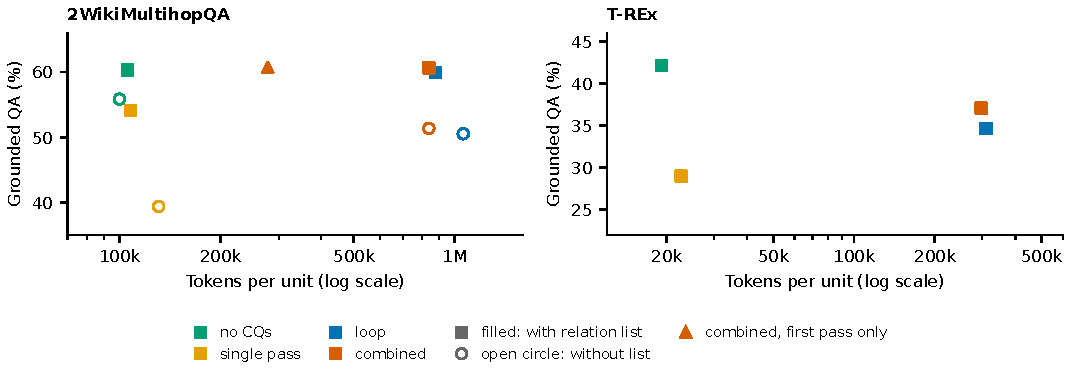
\includegraphics[width=\textwidth]{figures/fig_cost_quality_r64.pdf}
\caption{Seeded extraction without CQs was not distinguishable from the combined pipeline in grounded QA at a fraction of its tokens (106k against 838k per unit). Points are arm means of grounded QA against tokens per unit (log axis); intervals for the contrasts are in Tables~\ref{tab:glance} and~\ref{tab:itext}. Left, 2Wiki: arms with and without the list. Right, T-REx: seeded arms only. Qwen.}
\label{fig:costquality}
\end{figure*}}{}

The Exp7 arms on T-REx, every arm given the original 22 names, repeat the comparison on a second corpus. Seeded extraction scored .421 grounded QA against .371 for the combined pipeline, 5.0 points higher (registered 90\% interval [1.1, 8.1]), at 19.1k tokens per unit against 298k. Seeded extraction led, so the registered equivalence test at $\pm$3 points did not establish equivalence there.

\paragraph{Three public extractors in the same setup.}
None of the three public extractors received a relation list, and each ran with released defaults. Unseeded extraction, which also had no list, scored .558 grounded QA on the same units (Table~\ref{tab:exp8}). Run with Qwen on 2Wiki in the Exp7 setup (60 units, none failed), iText2KG wrote 1,899 facts, more than any arm in Table~\ref{tab:exp8}, and reached .430 grounded QA (Table~\ref{tab:itext}). That is 17.3 points below seeded extraction and 17.6 below the combined pipeline (both descriptive), at 478.8k tokens per unit against 105.9k and 837.7k. Against the single pass it was 3.7 points higher in grounded QA (interval includes zero) and 11.6 in answer correctness.
EDC, a second public extractor, induces its schema from the text and canonicalises it itself, and we ran it on the same model and engine with its released defaults (Self Canonicalization)~\cite{zhang2024edc}. It scored .445 grounded QA and .629 answer correctness (Table~\ref{tab:itext}), 5.1 points ([0.5, 10.0]) and 19.6 points ([14.8, 24.7]) above the single pass. EDC scored 15.8 points below seeded extraction in grounded QA ([$-$19.3, $-$12.3]; answer correctness $-$4.9 [$-$7.7, $-$2.5]), at 618.4k tokens per unit against 105.9k, and 16.1 points below the combined pipeline ([$-$20.1, $-$12.4]). EDC was also given the same 22-name list as its target schema, with the names as definitions (its Target Alignment mode), on the 30 units of one run seed; these arm means are on 30 units, so they differ from the 60-unit table values. It scored .458 grounded QA (.613 answer correctness) with the list against .454 (.633) without it, +0.4 points ([$-$2.7, 2.9], registered: not established), with 824 against 1,356 facts per unit. Seeded extraction scored 14.6 points above EDC with the list ([10.4, 18.5], registered: improved, Holm $p$ = 0.0003), so giving EDC the same list did not close the gap. All other differences involving EDC are descriptive.

AutoSchemaKG, a third public extractor, also induces its schema from the text~\cite{bai2026autoschemakg}. We ran it with its released defaults on the same model family, chunks, answerer and scorer, on 30 2Wiki shards with one run seed, and report the comparison as descriptive. Its entity-relation triples, the variant comparable to the other arms, scored .213 grounded QA and .446 answer correctness with 1,256.6 facts at 1,557.8k tokens per unit (Table~\ref{tab:itext}). On the same 30 shards, the stored seeded extraction scored .604 and .679, the combined pipeline .631 and .677, and the single pass .404 and .425. It scored 39.2 points below seeded extraction in grounded QA ([$-$44.0, $-$34.4]; answer correctness $-$23.3 [$-$27.5, $-$20.0]), and 41.9 points below the combined pipeline ([$-$46.3, $-$38.3]; $-$23.1 [$-$27.3, $-$19.0]). Against the single pass it scored 19.2 points lower in grounded QA ([$-$26.0, $-$13.1]), and the answer correctness difference was +2.1 ([$-$5.0, 9.4]; the interval includes zero).

Requiring a matching relation class changed each arm's grounded QA by at most 1.2 points and left the gaps unchanged or wider (post hoc reanalysis of the stored predictions). As a descriptive observation, the gold evidence pairs reached the 60 retrieved facts in 88.5\% of cases for seeded extraction, 81.0\% for iText2KG, 75.6\% for EDC and 57.7\% for AutoSchemaKG triples. Relaxing entity linking changed these reach rates by at most 0.5 points in every arm (post hoc, stored graphs).

\begin{table*}[t]
\centering
\caption{Three public extractors against Exp7 arms (Qwen, 2Wiki, 60 shard $\times$ run seed units; descriptive). EDC ran with its released defaults (Self Canonicalization). The AutoSchemaKG rows cover 30 shards with one run seed, and their differences are taken against the stored arms on those shards. AutoSchemaKG's entity-relation triples are the comparable variant; its full graph also holds concept and event edges. Tokens are per unit, in thousands. The difference rows give each extractor minus the arm, in points, with 95\% intervals.}
\label{tab:itext}
\footnotesize\setlength{\tabcolsep}{3pt}
\begin{tabular}{lcccc}
\toprule
 & Grounded QA & Answer correctness & Facts & Tokens (k) \\
\midrule
iText2KG & .430 [.393, .470] & .549 [.503, .596] & 1,899 & 478.8 \\
EDC & .445 [.398, .493] & .629 [.583, .676] & 1,357.7 & 618.4 \\
AutoSchemaKG, entity-relation triples & .213 [.175, .252] & .446 [.396, .490] & 1,256.6 & 1,557.8 \\
AutoSchemaKG, full graph & .096 [.073, .121] & .233 [.200, .260] & 18,360 & 1,557.8 \\
Seeded extraction & .603 & .678 & 1,472 & 105.9 \\
Combined & .606 & .655 & 1,435 & 837.7 \\
Single pass (L0) & .394 & .433 & 725 & 131.0 \\
\midrule
iText2KG $-$ seeded extraction & $-$17.3 [$-$21.0, $-$13.9] & $-$12.9 [$-$16.3, $-$10.0] & & \\
iText2KG $-$ combined & $-$17.6 [$-$20.8, $-$14.1] & $-$10.6 [$-$14.1, $-$7.5] & & \\
iText2KG $-$ single pass & $+$3.7 [$-$1.5, 9.3] & $+$11.6 [5.6, 18.2] & & \\
EDC $-$ seeded extraction & $-$15.8 [$-$19.3, $-$12.3] & $-$4.9 [$-$7.7, $-$2.5] & & \\
EDC $-$ combined & $-$16.1 [$-$20.1, $-$12.4] & $-$2.6 [$-$5.9, 0.5] & & \\
EDC $-$ single pass & $+$5.1 [0.5, 10.0] & $+$19.6 [14.8, 24.7] & & \\
AutoSchemaKG triples $-$ seeded extraction & $-$39.2 [$-$44.0, $-$34.4] & $-$23.3 [$-$27.5, $-$20.0] & & \\
AutoSchemaKG triples $-$ combined & $-$41.9 [$-$46.3, $-$38.3] & $-$23.1 [$-$27.3, $-$19.0] & & \\
AutoSchemaKG triples $-$ single pass & $-$19.2 [$-$26.0, $-$13.1] & $+$2.1 [$-$5.0, 9.4] & & \\
\bottomrule
\end{tabular}
\end{table*}

\paragraph{Retrieval over the same chunks.}
On the same 2Wiki units, seeded extraction reached .669 answer correctness in a rerun on the retrieval arms' own serving engine (.678 in the stored run, Table~\ref{tab:itext}). Retrieval-augmented generation from the top 5 chunks reached .515, and .500 with the 22-name list as a hint. Answer correctness is the common measure because the retrieval arms have no graph facts, so grounded QA cannot be computed for them. With no context, the answer model reached .325 from its own knowledge (descriptive); seeded extraction scored 35.3 points higher ([30.1, 40.1]). The graph scored 15.4 points above chunk retrieval ([10.6, 19.8]) and 16.9 above list-hinted retrieval ([11.1, 22.3]), and both comparisons were registered as improved.

The grounded-QA results above use graph facts only. When passages were added to the retrieved facts (hybrid QA) and the graph facts were capped at 60, every pipeline scored above vector-only QA (.502): LOOP+seed .725, L0+seed .716, U-ext+seed .709, Combined .699 and L0 .626 (60 units). Raising the fact cap from 30 to 60 raised U-ext+seed by 12.4 points ([9.3, 15.3]) and Combined by 9.6 ([7.2, 11.7]); both were registered as improved in answer correctness. In the stored run with up to 30 facts the scores were L0+seed .692, LOOP+seed .671, Combined .603, L0 .600 and U-ext+seed .585 (Appendix Table~\ref{tab:newchecks}): with 30 facts the arms with the most facts ranked lowest, and with 60 the four list or full-extraction arms were close. The cap was the setting we varied.

\section{What CQs Add: Each Fact Counts}
\label{sec:res-cqs}
\label{sec:res-coverage}

Two results on the equal-fact-count check come first. With the relation list, the guided single pass scored 39.1 points above an equal-size random subset of seeded extraction in grounded QA ([34.2, 44.1]); a registered test asked whether the random subset scores higher, and it did not. The lead held against further selectors, among them selections made with the CQs or balanced over chunks (below). Without the list the relation-frequency selection scored 8.0 points above the guided pass ([2.7, 13.3]; registered), and on T-REx without the list the contrast with a random subset was not established (6.6 points, [$-$5.8, 12.2]).

Without the list, U-ext raised grounded QA over L0 by 16.5 points ([10.6, 21.7], post hoc) by writing 1,704 facts against 725. The check compares the CQ-guided facts with facts chosen at random: we drew a uniform random subset of the stored U-ext graph (or of the listed graph, for the listed comparison) down to the fact count of the matching single pass, and the same answerer and scorer scored it. The plan was fixed before any model call. Without the list, the single pass scored 28.2 points above an equal-size random subset of open extraction ([23.4, 33.2]). On T-REx with the list, the single pass scored 7.4 points above an equal-size random subset of seeded extraction ([2.9, 12.8], Holm $p$ = 0.001, registered: improved). Two heuristic selections, one by relation frequency and one by entity centrality, cut the extraction graph to the guided graph's fact count. With the list, the CQ-guided single pass stayed ahead of both, by 16.6 points against the relation-frequency selection ([11.4, 22.1]) and 25.8 against the centrality selection ([20.5, 30.5]) in grounded QA (registered; Appendix Table~\ref{tab:selection}).

On 2Wiki with the list (60 units), the guided pass scored 25.0 points above the chain-preserving selector ([19.8, 30.1]) and 14.3 above the model selector ([8.9, 19.3]) in grounded QA (both registered: improved, Holm $p$ = 0.0002; Appendix Table~\ref{tab:selection}). Selections by the CQs of the unit and balanced over chunks scored below the guided pass by 33.3 points ([28.3, 37.7]) and 37.2 points ([31.6, 41.4]) in grounded QA (both registered: improved, Holm $p$ = 0.0004 and 0.0005). This separates CQ-guided extraction from CQ-guided selection.

CQs also leave a schema that answers structured queries. On 40 fresh CQs per shard and run seed, written from random chunks with a neutral prompt, the combined pipeline passed 13.5 points more through SPARQL than seeded extraction ([10.7, 16.3]).
